\documentclass[14pt]{extbook}
\usepackage{multicol, enumerate, enumitem, hyperref, color, soul, setspace, parskip, fancyhdr} %General Packages
\usepackage{amssymb, amsthm, amsmath, bbm, latexsym, units, mathtools} %Math Packages
\everymath{\displaystyle} %All math in Display Style
% Packages with additional options
\usepackage[headsep=0.5cm,headheight=12pt, left=1 in,right= 1 in,top= 1 in,bottom= 1 in]{geometry}
\usepackage[usenames,dvipsnames]{xcolor}
\usepackage{dashrule}  % Package to use the command below to create lines between items
\newcommand{\litem}[1]{\item#1\hspace*{-1cm}\rule{\textwidth}{0.4pt}}
\pagestyle{fancy}
\lhead{Progress Quiz 10}
\chead{}
\rhead{Version A}
\lfoot{6232-9639}
\cfoot{}
\rfoot{Fall 2020}
\begin{document}

\begin{enumerate}
\litem{
Determine the domain of the function below.\[ f(x) = \frac{3}{36x^{2} +12 x -15} \]\begin{enumerate}[label=\Alph*.]
\item \( \text{All Real numbers except } x = a, \text{ where } a \in [-30.2, -27.8] \)
\item \( \text{All Real numbers.} \)
\item \( \text{All Real numbers except } x = a \text{ and } x = b, \text{ where } a \in [-30.2, -27.8] \text{ and } b \in [17.9, 19.9] \)
\item \( \text{All Real numbers except } x = a, \text{ where } a \in [-2.8, -0.6] \)
\item \( \text{All Real numbers except } x = a \text{ and } x = b, \text{ where } a \in [-2.8, -0.6] \text{ and } b \in [-0.5, 1.6] \)

\end{enumerate} }
\litem{
Choose the equation of the function graphed below.
\begin{center}
    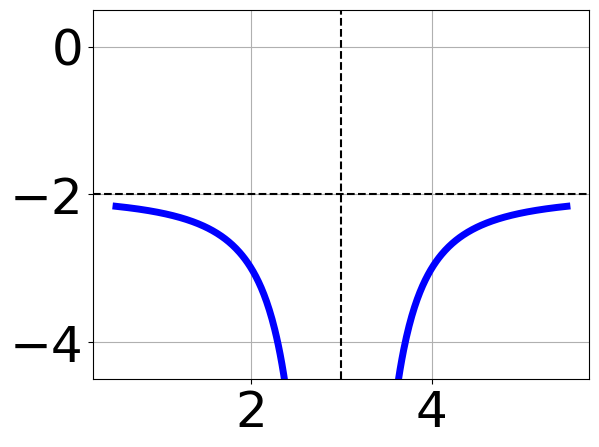
\includegraphics[width=0.5\textwidth]{../Figures/rationalGraphToEquationA.png}
\end{center}
\begin{enumerate}[label=\Alph*.]
\item \( f(x) = \frac{-1}{x - 3} - 2 \)
\item \( f(x) = \frac{-1}{(x - 3)^2} - 2 \)
\item \( f(x) = \frac{1}{x + 3} - 2 \)
\item \( f(x) = \frac{1}{(x + 3)^2} - 2 \)
\item \( \text{None of the above} \)

\end{enumerate} }
\litem{
Solve the rational equation below. Then, choose the interval(s) that the solution(s) belongs to.\[ \frac{6x}{6x + 4} + \frac{-4x^{2}}{42x^{2} +40 x + 8} = \frac{7}{7x + 2} \]\begin{enumerate}[label=\Alph*.]
\item \( x_1 \in [-0.99, -0.54] \text{ and } x_2 \in [1.34,5.34] \)
\item \( x \in [0.95,1.53] \)
\item \( x_1 \in [-0.99, -0.54] \text{ and } x_2 \in [-5.67,0.33] \)
\item \( \text{All solutions lead to invalid or complex values in the equation.} \)
\item \( x \in [-0.3,0.15] \)

\end{enumerate} }
\litem{
Solve the rational equation below. Then, choose the interval(s) that the solution(s) belongs to.\[ \frac{3}{-4x + 8} + 3 = \frac{6}{32x -64} \]\begin{enumerate}[label=\Alph*.]
\item \( x \in [-2.06,-1.42] \)
\item \( x_1 \in [-2.06, -1.42] \text{ and } x_2 \in [0.31,3.31] \)
\item \( x_1 \in [1.28, 2.15] \text{ and } x_2 \in [0.31,3.31] \)
\item \( \text{All solutions lead to invalid or complex values in the equation.} \)
\item \( x \in [1.31,4.31] \)

\end{enumerate} }
\litem{
Choose the graph of the equation below.\[ f(x) = \frac{-1}{x - 2} - 2 \]\begin{enumerate}[label=\Alph*.]
\begin{multicols}{2}\item 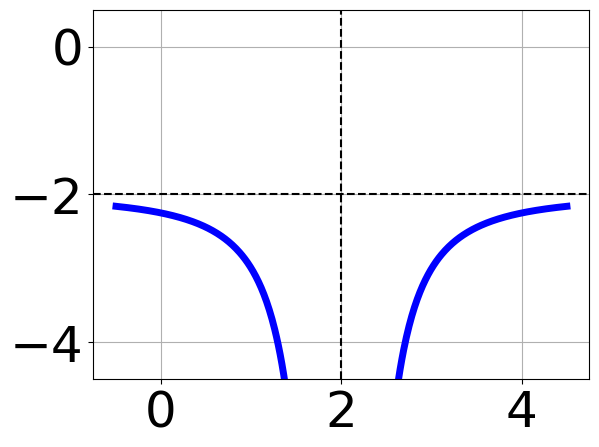
\includegraphics[width = 0.3\textwidth]{../Figures/rationalEquationToGraphAA.png}\item 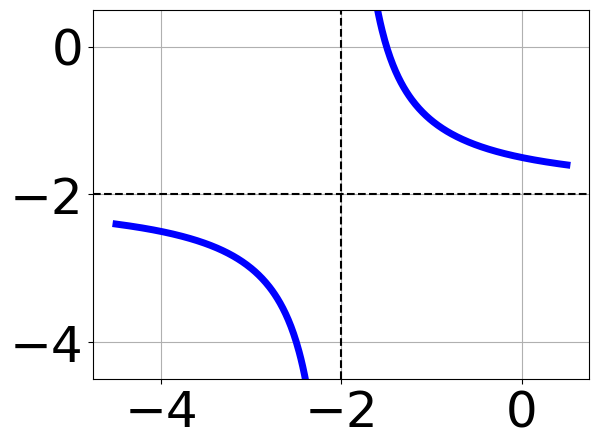
\includegraphics[width = 0.3\textwidth]{../Figures/rationalEquationToGraphBA.png}\item 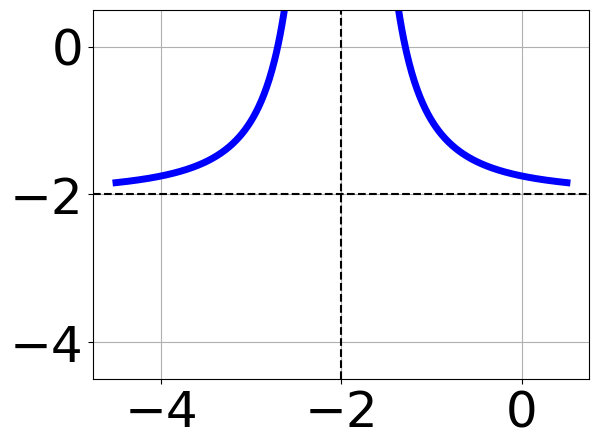
\includegraphics[width = 0.3\textwidth]{../Figures/rationalEquationToGraphCA.png}\item 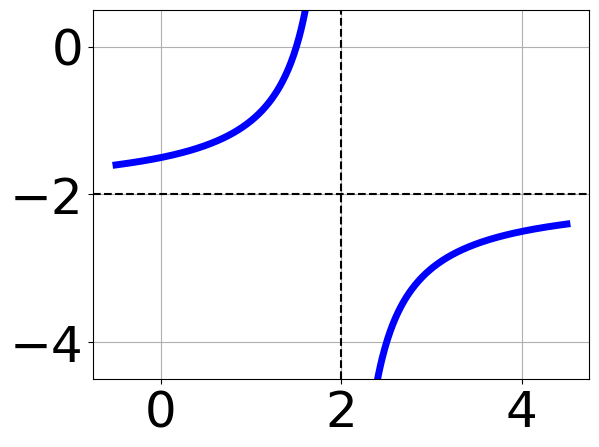
\includegraphics[width = 0.3\textwidth]{../Figures/rationalEquationToGraphDA.png}\end{multicols}\item None of the above.
\end{enumerate} }
\litem{
Solve the rational equation below. Then, choose the interval(s) that the solution(s) belongs to.\[ \frac{-84}{60x + 60} + 1 = \frac{-84}{60x + 60} \]\begin{enumerate}[label=\Alph*.]
\item \( x_1 \in [-1.6, -0.7] \text{ and } x_2 \in [-1.1,0.3] \)
\item \( \text{All solutions lead to invalid or complex values in the equation.} \)
\item \( x_1 \in [-1.6, -0.7] \text{ and } x_2 \in [-0.3,1.4] \)
\item \( x \in [-1.0,1.0] \)
\item \( x \in [0.4,1.9] \)

\end{enumerate} }
\litem{
Determine the domain of the function below.\[ f(x) = \frac{3}{18x^{2} -24 x -24} \]\begin{enumerate}[label=\Alph*.]
\item \( \text{All Real numbers except } x = a, \text{ where } a \in [-25, -22] \)
\item \( \text{All Real numbers except } x = a, \text{ where } a \in [-0.67, 0.33] \)
\item \( \text{All Real numbers except } x = a \text{ and } x = b, \text{ where } a \in [-25, -22] \text{ and } b \in [18, 19] \)
\item \( \text{All Real numbers.} \)
\item \( \text{All Real numbers except } x = a \text{ and } x = b, \text{ where } a \in [-0.67, 0.33] \text{ and } b \in [1, 5] \)

\end{enumerate} }
\litem{
Choose the graph of the equation below.\[ f(x) = \frac{-1}{x - 2} + 2 \]\begin{enumerate}[label=\Alph*.]
\begin{multicols}{2}\item 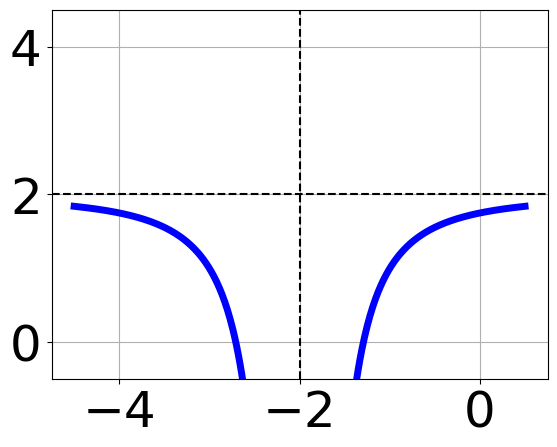
\includegraphics[width = 0.3\textwidth]{../Figures/rationalEquationToGraphCopyAA.png}\item 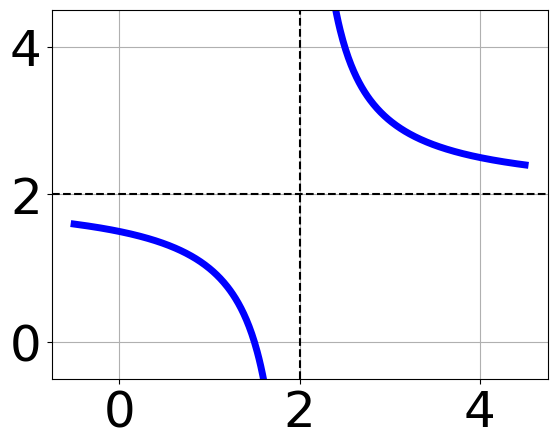
\includegraphics[width = 0.3\textwidth]{../Figures/rationalEquationToGraphCopyBA.png}\item 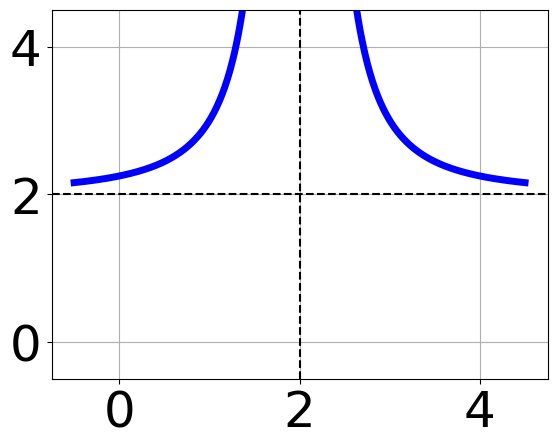
\includegraphics[width = 0.3\textwidth]{../Figures/rationalEquationToGraphCopyCA.png}\item 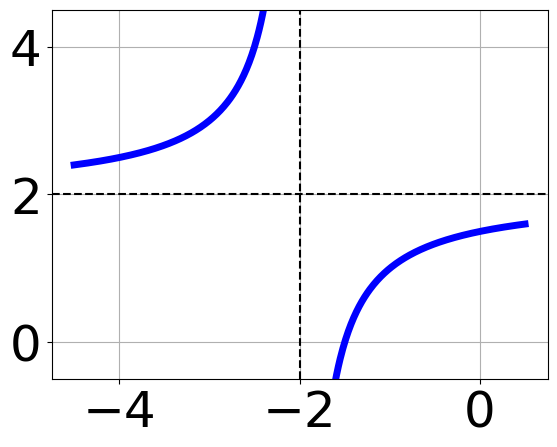
\includegraphics[width = 0.3\textwidth]{../Figures/rationalEquationToGraphCopyDA.png}\end{multicols}\item None of the above.
\end{enumerate} }
\litem{
Choose the equation of the function graphed below.
\begin{center}
    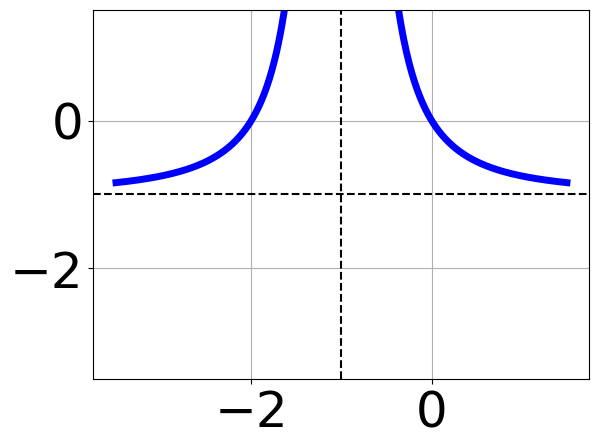
\includegraphics[width=0.5\textwidth]{../Figures/rationalGraphToEquationCopyA.png}
\end{center}
\begin{enumerate}[label=\Alph*.]
\item \( f(x) = \frac{1}{(x + 1)^2} - 1 \)
\item \( f(x) = \frac{-1}{(x - 1)^2} - 1 \)
\item \( f(x) = \frac{1}{x + 1} - 1 \)
\item \( f(x) = \frac{-1}{x - 1} - 1 \)
\item \( \text{None of the above} \)

\end{enumerate} }
\litem{
Solve the rational equation below. Then, choose the interval(s) that the solution(s) belongs to.\[ \frac{-6x}{-5x -4} + \frac{-4x^{2}}{15x^{2} -23 x -28} = \frac{-4}{-3x + 7} \]\begin{enumerate}[label=\Alph*.]
\item \( x_1 \in [-1.22, 1.87] \text{ and } x_2 \in [-0.8,0.2] \)
\item \( x_1 \in [-1.22, 1.87] \text{ and } x_2 \in [4.67,6.67] \)
\item \( x \in [1.37,4.17] \)
\item \( \text{All solutions lead to invalid or complex values in the equation.} \)
\item \( x \in [3.16,6.6] \)

\end{enumerate} }
\end{enumerate}

\end{document}